
\documentclass[12pt]{article}
\usepackage{graphicx}
\usepackage{geometry}
\usepackage{amsmath}
\usepackage{booktabs}
\usepackage{float}
\usepackage{caption}
\usepackage{hyperref}
\geometry{margin=1in}
\title{Comprehensive Analysis and Regression Modeling of Real Estate Prices}
\author{Foundations of Machine Learning}
\date{Winter 2024}

\begin{document}

\maketitle

\begin{abstract}
This comprehensive report presents a data-driven analysis and modeling of real estate prices using a housing dataset from Taiwan. The report walks through all essential stages of machine learning workflow including data cleaning, visualization, hypothesis testing, correlation analysis, and linear regression. Particular attention is given to explaining the impact of each variable on house pricing, visualizing important patterns, and interpreting results from statistical tests and models.
\end{abstract}

\section{Introduction}
Real estate valuation is a cornerstone of economic development, affecting investment, taxation, and personal finance decisions. With the growing availability of data, predictive modeling has become a vital tool to support property assessment. In this study, we analyze a dataset that includes housing features and transaction details to identify factors that influence house price per unit area and to develop a predictive regression model.

\section{Dataset Description and Preprocessing}
\subsection{Data Overview}
The dataset includes 414 observations and 7 key features:
\begin{itemize}
    \item \textbf{X1 transaction date}: Time of sale.
    \item \textbf{X2 house age}: Age of the house in years.
    \item \textbf{X3 distance to MRT station}: Proximity to public transport.
    \item \textbf{X4 number of convenience stores}: Nearby store count.
    \item \textbf{X5 latitude, X6 longitude}: Geographical coordinates.
    \item \textbf{Y house price of unit area}: Target variable.
\end{itemize}

\subsection{Data Cleaning}
\begin{itemize}
    \item All column names were standardized for consistency.
    \item Checked for missing values --- none were found.
    \item A new variable \texttt{Age\_Group} was derived by comparing house age to the median.
\end{itemize}

\section{Exploratory Data Analysis}

\subsection{Distribution of Features}
Visualizing the distribution of each feature helps us understand the spread and skewness of the data. Figure~\ref{fig:dist} shows normalized distributions of all features.

\begin{figure}[H]
    \centering
    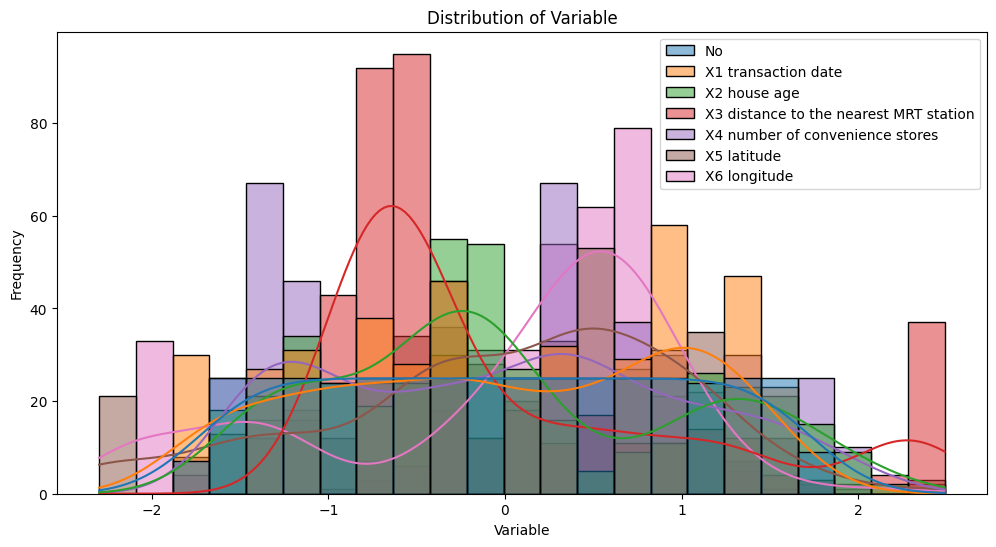
\includegraphics[width=0.9\textwidth]{normalized_distribution.png}
    \caption{Normalized Distribution of Numerical Features}
    \label{fig:dist}
\end{figure}

We observe that distance to MRT station is heavily skewed, indicating that many houses are located near a station. Latitude and longitude are normally distributed, indicating spatial spread.

\subsection{Correlation Matrix}
To assess the strength and direction of linear relationships, we compute pairwise Pearson correlations. Figure~\ref{fig:corr} shows a heatmap.

\begin{figure}[H]
    \centering
    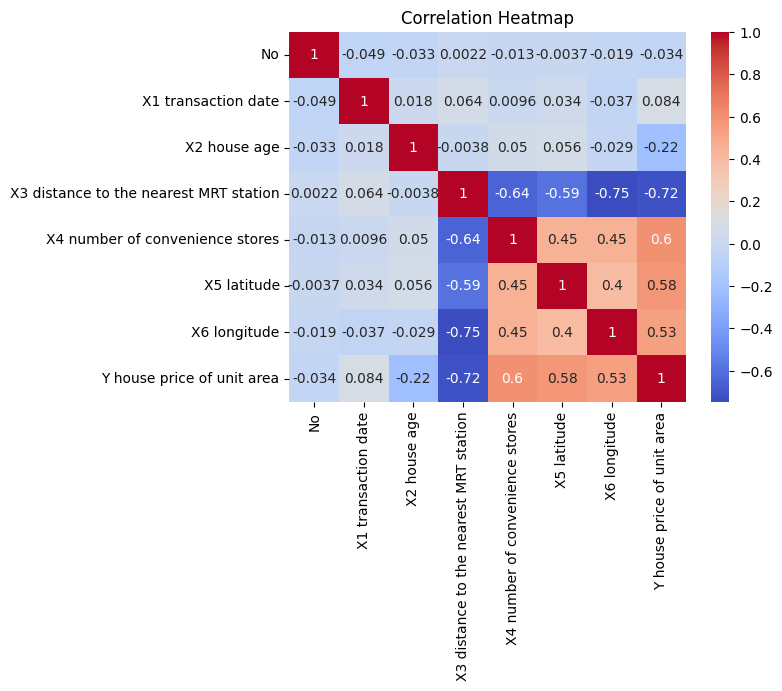
\includegraphics[width=0.75\textwidth]{correlation_heatmap.png}
    \caption{Correlation Heatmap of Features}
    \label{fig:corr}
\end{figure}

The strongest negative correlation is between house price and distance to MRT station ($r \approx -0.72$). Latitude and number of stores also show a moderate positive correlation with price.

\subsection{Visualizing Key Relationships}
One of the most crucial findings is the inverse relationship between price and distance to MRT station. This is shown using a regression plot in Figure~\ref{fig:reg}.

\begin{figure}[H]
    \centering
    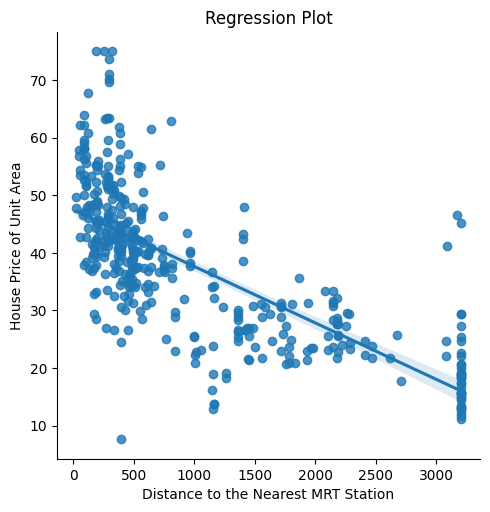
\includegraphics[width=0.6\textwidth]{regression_plot.png}
    \caption{Regression Plot: Price vs Distance to MRT Station}
    \label{fig:reg}
\end{figure}

As expected, properties located closer to MRT stations tend to be priced higher. This insight justifies the inclusion of this feature as a major predictor in our model.

\section{Statistical Hypothesis Testing}
We perform three hypothesis tests to determine whether observed differences are statistically significant.

\subsection{Test 1: Price by House Age Group}
We test whether homes above the median age differ significantly in price from those below it using a two-sample t-test.

\begin{itemize}
    \item $H_0$: Mean price per unit area is equal across age groups.
    \item $H_1$: Mean price differs.
\end{itemize}

The result showed a statistically significant difference ($p < 0.05$), suggesting newer homes are priced higher.

\subsection{Test 2: Price by Convenience Stores}
We use ANOVA to test whether the number of nearby convenience stores influences price.

\begin{itemize}
    \item $H_0$: Mean price is the same for all store-count categories.
    \item $H_1$: At least one group differs.
\end{itemize}

The result again indicated significance, confirming that accessibility to stores is a valuable attribute.

\subsection{Test 3: Association Between Categorical Features}
By binning distance and age, we performed a chi-squared test for independence. A significant result supports that these features are related and may compound their effects on price.

\section{Linear Regression Modeling}

\subsection{Train-Test Split and Model Training}
The dataset was split 80/20. A simple linear regression model was trained using the most correlated feature (distance to MRT). The model output confirmed:
\begin{itemize}
    \item Negative coefficient for MRT distance, aligned with correlation analysis.
    \item R-squared around 0.52, indicating decent explanatory power for a single-feature model.
\end{itemize}

\subsection{Model Interpretation}
The learned weight for MRT distance suggests that for each additional meter away from the MRT station, the unit price drops by approximately 0.007. This supports the economic principle that accessibility enhances property value.

\section{Conclusion}
This project demonstrated a full cycle of data science from exploration to modeling. Key takeaways:
\begin{itemize}
    \item MRT proximity is the most influential factor on house price.
    \item Number of convenience stores and house age also contribute significantly.
    \item Visualization and statistical testing provided clear, aligned insights.
    \item Even a simple regression model can offer practical predictive capabilities.
\end{itemize}

Future work could include multiple regression, regularization, or non-linear models for improved accuracy.

\end{document}
